\chapter{Project Overview}

\section{Project Title and Description}
The project developed during this industrial attachment is titled the \textbf{URL Shrinker API}. It is a high-performance, production-grade URL shortening web service consisting of a Go-based REST API backend and a Next.js React frontend. The primary purpose of a URL shortener is to convert long, cumbersome web addresses (URLs) into compact, manageable aliases (short codes). When a user navigates to the short URL, the system redirects them to the original destination URL. 

Beyond core redirection, the URL Shrinker API provides:
\begin{itemize}
    \item \textbf{User Management \& Authentication:} Secure signup and login powered by JWT with refresh token rotation.
    \item \textbf{Link Customization:} Options to define custom short codes or generate random secure codes.
    \item \textbf{Link Expiration \& Control:} Setting maximum click limits, expiration timestamps, or manual deactivation.
    \item \textbf{Analytics Dashboard:} Real-time click tracking, recording user-agent information, IP addresses, referrers, and request timestamps.
    \item \textbf{Automated Housekeeping:} A background cleanup worker that removes expired links to optimize database storage.
\end{itemize}

\section{Problem Identification and Complexity Analysis}
At first glance, a URL shortener appears to be a trivial software system. However, operating such a service at scale reveals significant software engineering challenges and architectural complexities:

\subsection{Read-to-Write Ratio Imbalance}
URL shorteners experience an extremely high ratio of read requests (redirects) compared to write requests (creating new short links). A single viral short link can receive millions of hits in a few minutes. Querying a relational database (PostgreSQL) directly for every single redirect request creates severe I/O bottlenecks, degrades response times, and can lead to database connection pool exhaustion.
\textbf{Complexity Solution:} Implementing a high-speed caching layer (Redis) using the \textbf{Cache-Aside pattern}. Redirection requests are served directly from memory, maintaining low latency (sub-10ms).

\subsection{Short Code Generation \& Collision Handling}
The system must generate short, unique strings (typically 6–8 characters). Generating a random string and checking if it exists in the database before insertion can result in multiple expensive database checks as the database grows, known as the "collision check loop."
\textbf{Complexity Solution:} Generating unique random codes using secure pseudo-random characters (Base62 character set: `a-z`, `A-Z`, `0-9`) and handling collisions using transaction-level constraints and sentinel error catches.

\subsection{Link Expiration and Database Bloat}
If thousands of temporary short links are created, the database size grows continuously. Old, expired links will clutter database pages, slow down database indexing, and increase hosting costs.
\textbf{Complexity Solution:} Incorporating a background worker routine in Go using a time ticker that runs an SQL garbage collection script periodically (e.g., hourly) to delete expired links and their associated analytics records, maintaining database hygiene.

\section{Literature Survey and Background Study}
To design the URL Shrinker API, a study of existing systems (such as Bitly and TinyURL) and technical standards was conducted:

\subsection{Redirection HTTP Semantics}
There are two main HTTP redirect codes used for URL shortening, each with distinct caching implications:
\begin{itemize}
    \item \textbf{HTTP 301 (Moved Permanently):} The client browser caches this redirect. Subsequent visits to the short URL will skip the shortening server and go straight to the target URL.
    \item \textbf{HTTP 302 (Found / Temporary Redirect):} The browser does not cache this redirect. Every click on the short URL is forced to pass through the shortening server first.
\end{itemize}
\textbf{Conclusion:} The URL Shrinker API uses **HTTP 302**. While HTTP 301 reduces server load by offloading redirection to the client, it makes click analytics tracking impossible. Using HTTP 302 ensures every request hits our middleware, allowing us to record accurate, real-time click statistics before redirecting the client.

\subsection{Short Code Encoding Techniques}
There are two primary methods to generate short codes:
\begin{enumerate}
    \item \textbf{Base62 Encoding of Auto-increment IDs:} Convert the database auto-increment integer ID into a Base62 string (e.g., ID `100000` becomes `q0U`). 
    \item \textbf{Random Secure String Generation:} Generate a random string of fixed length (e.g., 6 characters) and store it as a key.
\end{enumerate}
Our implementation adopts random secure string generation. While Base62 encoding of sequential IDs is easy to implement, it makes the system predictable—users can guess other short URLs simply by incrementing or decrementing the short code. Secure random string generation prevents enumeration attacks.

\section{Problem-Solving Approach}
The system uses a clean, decoupled multi-layered architecture to separate concerns and ensure maintainability.

\subsection{Layered System Architecture}
The system is divided into distinct layers:
\begin{itemize}
    \item \textbf{HTTP Routing \& Middleware:} Manages HTTP requests, CORS headers, logging, JWT verification, and Redis-based rate limiting.
    \item \textbf{Handlers:} Decodes incoming JSON request payloads, validates input data, calls services, and formats JSON responses using a uniform enveloper.
    \item \textbf{Services:} Implements domain-specific business logic (e.g., verifying if a custom code is available, checking if a link has expired, managing refresh tokens).
    \item \textbf{Repositories:} Interfaces that bridge business logic to database queries and caching layers. This isolates the service layer from SQL/Redis driver dependencies.
    \item \textbf{Database \& Cache:} PostgreSQL for persistence and Redis for cache/rate-limiting keys.
\end{itemize}

The interaction between these system components is visualized in Figure~\ref{fig:system_architecture}.

\begin{figure}[htbp]
    \centering
    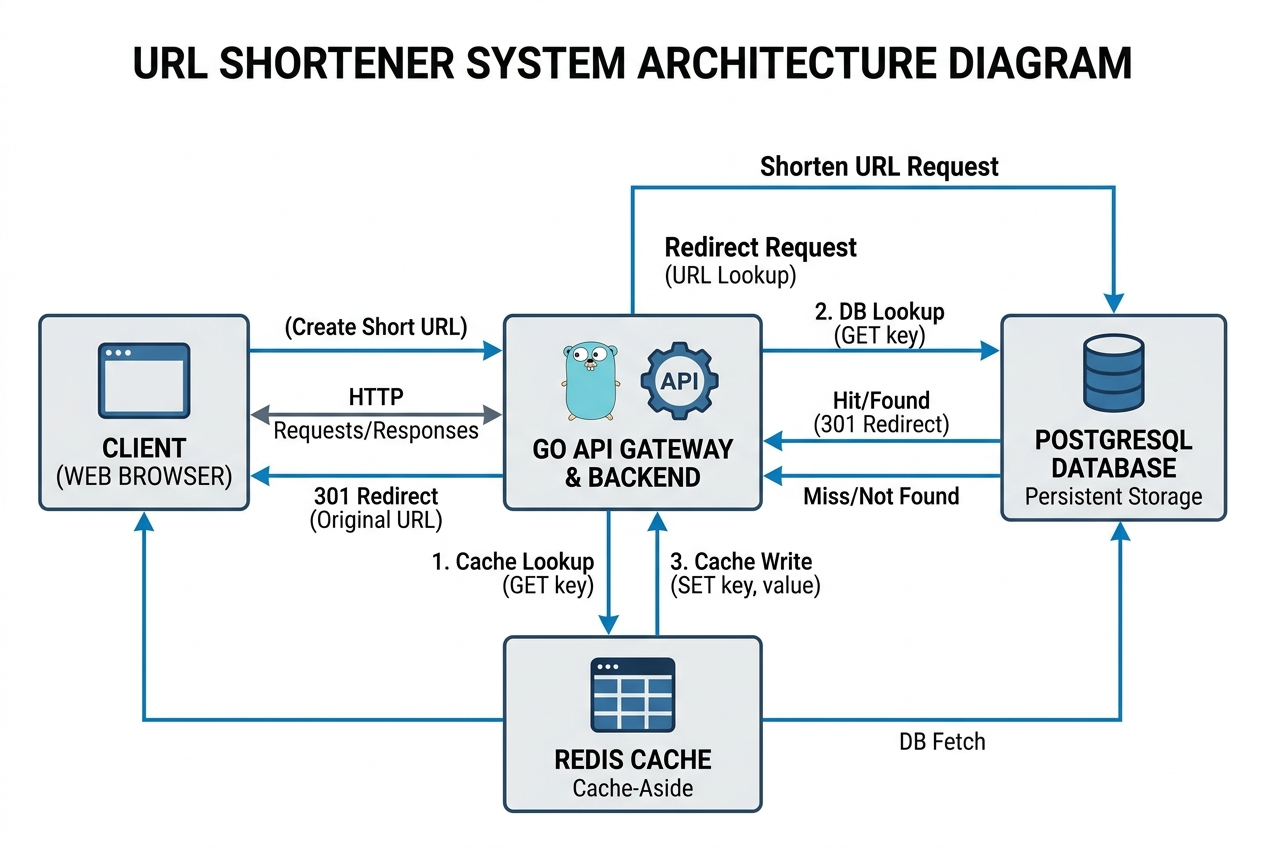
\includegraphics[width=0.85\textwidth]{images/system_architecture.jpg}
    \caption{URL Shortener System Architecture and Redirection Flow}
    \label{fig:system_architecture}
\end{figure}

\section{Experiment and Design Methodology}
The database schema and caching strategies were designed to support fast redirection:

\subsection{Database Schema Design}
The relational database consists of three main tables: `users`, `urls`, and `clicks` (analytics).
\begin{enumerate}
    \item \textbf{users:} Stores credentials (hashed using bcrypt) and token metadata.
    \item \textbf{urls:} Stores the original URL, short code, owner ID (optional, for anonymous/registered users), maximum click limit, expiration timestamp, status (active/inactive), and click count.
    \item \textbf{clicks:} Records redirect metrics (IP address, user-agent, referrer, timestamp) linked back to the `urls` table via a foreign key.
\end{enumerate}

To ensure fast lookup speeds, an index is explicitly created on the `code` column of the `urls` table, which is the primary query key during redirection. Detailed field mappings are shown in Table~\ref{tab:database_schema}.

\begin{table}[htbp]
    \centering
    \caption{Database Schema Details for Key Tables}
    \label{tab:database_schema}
    \begin{tabular}{llll}
        \toprule
        \textbf{Table} & \textbf{Column} & \textbf{Data Type} & \textbf{Constraints} \\
        \midrule
        \textbf{users} & id & SERIAL / INT & Primary Key \\
                       & email & VARCHAR(255) & Unique, Not Null \\
                       & password\_hash & VARCHAR(255) & Not Null \\
        \midrule
        \textbf{urls}  & id & SERIAL / INT & Primary Key \\
                       & original\_url & TEXT & Not Null \\
                       & code & VARCHAR(10) & Unique, Indexed, Not Null \\
                       & max\_clicks & INT & Default NULL \\
                       & expires\_at & TIMESTAMP & Default NULL \\
                       & is\_active & BOOLEAN & Default TRUE \\
        \midrule
        \textbf{clicks} & id & SERIAL & Primary Key \\
                       & url\_id & INT & Foreign Key (urls.id) ON DELETE CASCADE \\
                       & ip\_address & VARCHAR(45) & Not Null \\
                       & user\_agent & TEXT & Not Null \\
                       & clicked\_at & TIMESTAMP & Not Null \\
        \bottomrule
    \end{tabular}
\end{table}

\subsection{Cache-Aside Strategy Flowchart}
The logic for handling public URL redirection follows the Cache-Aside architecture:
\begin{enumerate}
    \item A request arrives at `/r/{code}`.
    \item The redirection handler queries Redis for the key `url:{code}`.
    \item \textbf{Cache Hit:} If the short code is found in Redis, the system decodes the JSON payload, records click metrics in a non-blocking background goroutine, and returns an HTTP 302 redirect.
    \item \textbf{Cache Miss:} If the code is not found in Redis:
    \begin{enumerate}
        \item The system queries PostgreSQL.
        \item If it does not exist, it returns an HTTP 404.
        \item If it exists, the system checks if the link is expired, deactivated, or has exceeded its maximum click limit. If invalid, it returns `410 Gone`.
        \item If valid, the system writes the URL payload to Redis with a Time-To-Live (TTL) (e.g., 24 hours) for future requests, records click metrics, and redirects the client.
    \end{enumerate}
\end{enumerate}

\section{Validation of Findings}
During testing in a local Docker container environment, the redirection API was validated for performance and correctness:
\begin{itemize}
    \item \textbf{Latency validation:} Redirection requests hitting the Redis cache returned responses in under **2–5 ms**, whereas requests querying PostgreSQL directly took **15–30 ms**.
    \item \textbf{Rate Limiting validation:} Attempts to trigger redirections or API creation beyond the set rate limit (e.g., 10 requests per minute) correctly returned an HTTP `429 Too Many Requests` status, with the header `Retry-After` specifying when the user could retry.
    \item \textbf{Automatic Cleanup validation:} Setting short links to expire within a minute and running the background worker verified that expired rows and their cascading analytics records were correctly deleted from PostgreSQL and evicted from Redis.
\end{itemize}
